\documentclass[12pt]{article}
\usepackage[utf8]{inputenc}
\usepackage{amsmath}
\usepackage{fancyhdr}
\usepackage{graphicx}
\usepackage{epstopdf}

\setlength{\oddsidemargin}{0in}
\setlength{\evensidemargin}{0in}
\setlength{\textwidth}{6.5in}
\setlength{\topmargin}{-.3in}
\setlength{\textheight}{9in}


\pagestyle{fancy}
\begin{document}

\begin{center}
{\Large Machine Learnig Homework 8} \\[.3in]
\end{center}
\lhead{Adam Kosiorek}
\rhead{IMAT: 03661883}
\vspace*{.5in}


\section*{Problem 1}

The k-nearest neighbours algorithm in the feature space by introducing the feature map is 

\begin{equation}
|\phi(x) - \phi(x^{(s_i)})|_2.
\label{eq:}
\end{equation}

In order that it only depends on the scalar product in feature space $K(\phi(x),\phi(x^{(s_i)})) = \phi(x)^T\phi(y)$, we square this. Using that operation, the k-nearest neighbours don't change.


\begin{align}
|\phi(x) - \phi(x^{(s_i)})|_2^2 =& (\phi(x) - \phi(x^{(s_i)}))^T(\phi(x) - \phi(x^{(s_i)})) \\
=& \phi(x)^T\phi(x) -2\phi(x)^T\phi(x^{(s_i)}) + \phi(x^{(s_i)})^T\phi(x^{(s_i)}).
\label{eq:}
\end{align}


When searching for the k training samples that minimize this function, the first term stays constant. Therefore, we can drop the term and must find k training samples $x^{(s_i)}$ that minimize 

\begin{equation}
 \phi(x^{(s_i)})^T\phi(x^{(s_i)})-2\phi(x)^T\phi(x^{(s_i)}) = K(x^{(s_i)}, x^{(s_i)}) - 2K(x, x^{(s_i)}).
\end{equation}

\section*{Problem 2}

The definition for a convex function is 

\begin{equation}
f(\alpha x + (1-\alpha)y) \leq \alpha f(x) +(1-\alpha)f(y).
\end{equation}

Plugging this into $h(x) = f(x)+g(x)$, gives us

\begin{align}
h(\alpha x + (1-\alpha)y) =& f(\alpha x + (1-\alpha)y) + g(\alpha x + (1-\alpha)y)\\
\leq& \alpha f(x) +(1-\alpha)f(y) +\alpha g(x) +(1-\alpha)g(y)\\
=& \alpha h(x) +(1-\alpha)h(y).
\end{align}

The proof of the scaled function being convex is

\begin{align}
u(\alpha x + (1-\alpha)y) =& cf(\alpha x + (1-\alpha)y)\\
\leq& c\left(\alpha f(x) +(1-\alpha)f(y)\right)\\
=& \alpha u(x) +(1-\alpha)u(y)
\end{align}

\section*{Problem 3}

By definition of convexity for every $\lambda$ we have for arbitrary x,y and $0\leq\alpha\leq1$

\begin{equation}
f_\lambda((1-\alpha)x + \alpha y) \leq (1-\alpha)f_\lambda(x) + \alpha f_\lambda(y).
\end{equation}

By definition of maximum we have

\begin{equation}
(1-\alpha)\max\limits_{\lambda}f_\lambda(x) + \alpha \max\limits_{\lambda}f_\lambda(y) \geq (1-\alpha)f_{\lambda '}(x) + \alpha f_{\lambda '}(y)
\end{equation}

for any $\lambda '$, which is the maximizer of $f_\lambda((1-\alpha)x + \alpha y)$ w.r.t. $\lambda$. We obtain

\begin{align}
(1-\alpha)f_{\lambda '}(x) + \alpha f_{\lambda '}(y) \geq& f_{\lambda '}(1-\alpha)x + \alpha y)\\
=& \max\limits_{\lambda}f_\lambda((1-\alpha)(x + \alpha y).
\end{align}

\section*{Problem 4}
The Lagrangian is given by

\begin{equation}
L(x,\alpha) = f_0(x) + \sum_{i}{\alpha_i f_i(x)}.
\end{equation}

This can also be interpreted as a family of functions $L_x(\alpha) = L(x,\alpha)$, that means we interpret $x$ as fixed. Thus $L_x(\alpha)$ has the form

\begin{equation}
L_x(\alpha) = C_{0,x} + \sum_{i}{C_{i,x} \alpha_i},
\end{equation}

where the $Cs$ are constants. By applying the definition of a convex function we see immediately that $L_x(\alpha)$ is convex for any $Cs$.
The Lagrange dual function is given by the pointwise minimum of this family of functions,

\begin{equation}
g(\alpha) = \min\limits_{x}L_x(\alpha) = -\max\limits_{x}(-L_x(\alpha)).
\end{equation}

The negative Lagragian $-L_x(\alpha)$ is also convex, because the negation only changes the sign of the
constants $C_{0,x}$ and $C_{i,x}$. Thus, as shown in the previous exercise,$-g(\alpha)$ is convex and $g(\alpha)$ is concave.

\section*{Problem 5}

\begin{figure}[ht]
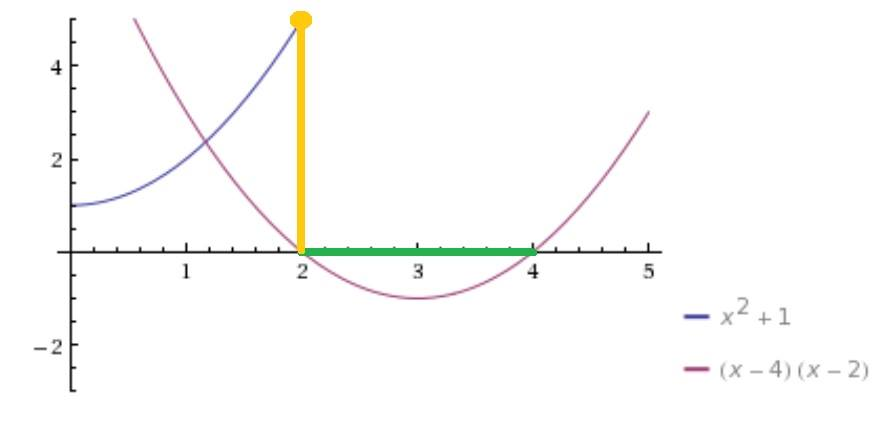
\includegraphics[width=\textwidth]{ex5.jpg}
\caption{The objective $f_0(x)$ and its constraint $f_1(x)$.}
\label{optimizationprob}
\end{figure}

The feasible region is marked green which is from 2 to 4 and the solution of the optimization problem is 2, also called the minimizer. In figure \ref{optimizationprob} the minimizer is marked orange.

\section*{Problem 6}

\begin{equation}
 \begin{align}
  L(x, \alpha) &= f_0(x) + \alpha f_1(x) \\
    &= x^2 + 1 + \alpha (x-2)(x-4) \\
    &= (1 + \alpha) x^2 - 6 \alpha x + (1 + 8 \alpha)
 \end{align}
\end{equation}



\begin{figure}[!ht] 
 \center
 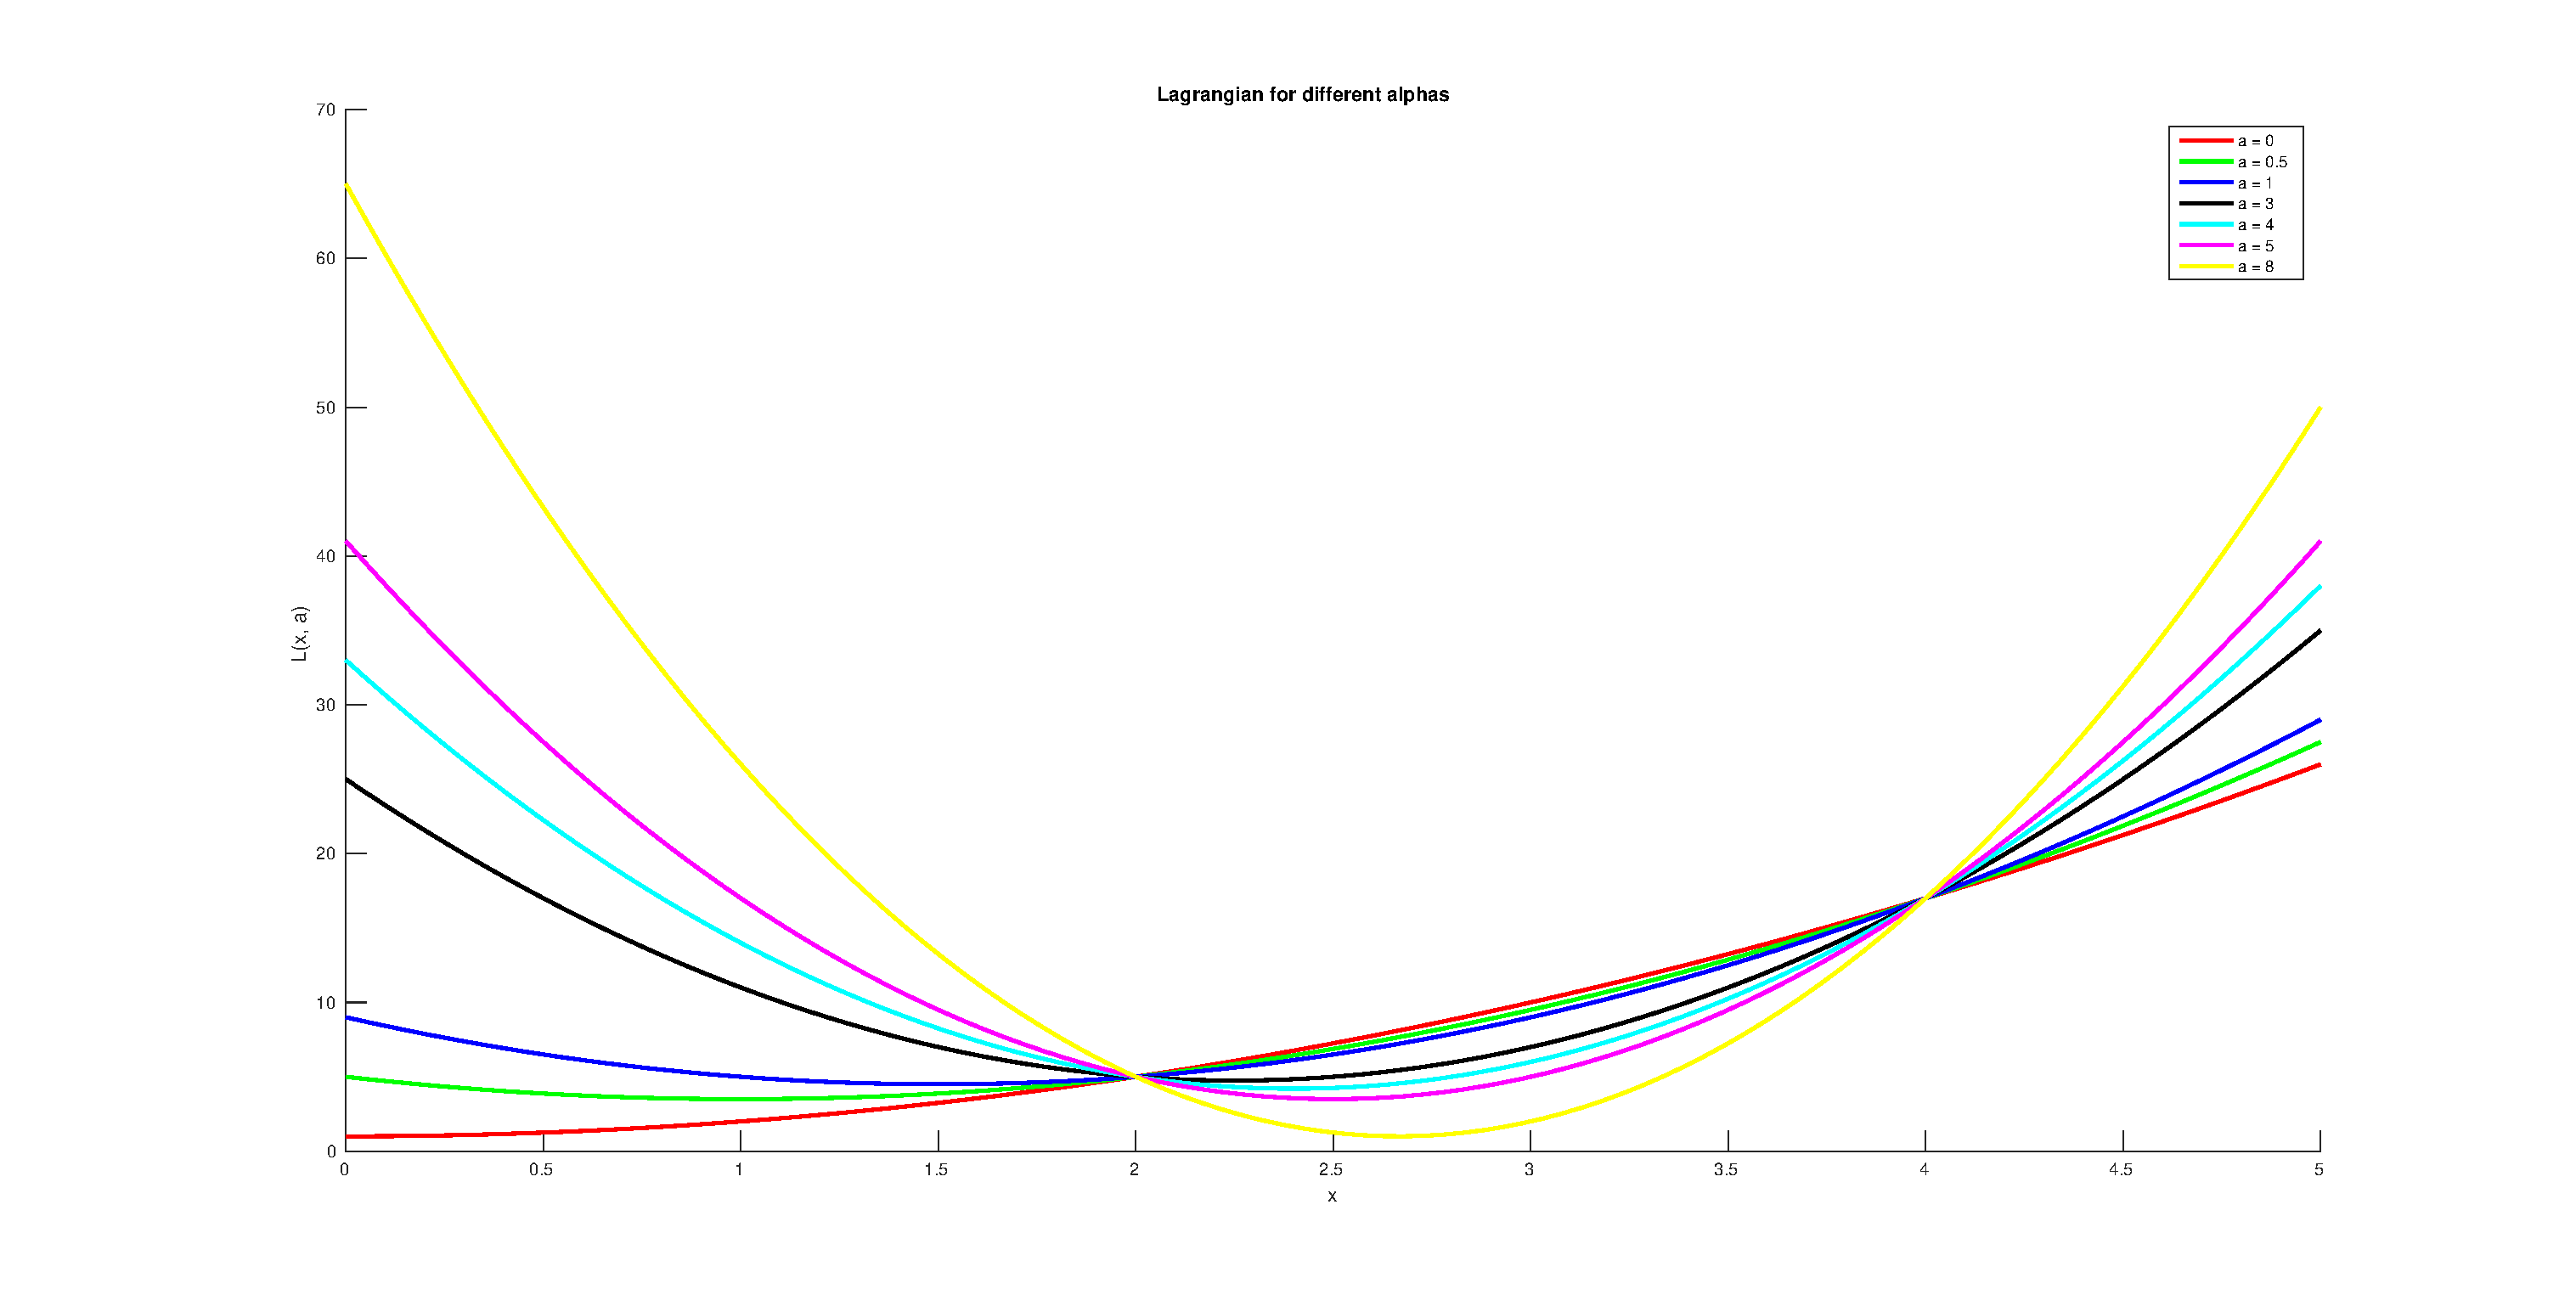
\includegraphics[width=\textwidth]{prob6}
 \caption{Lagrangian $L(x, \alpha)$ for different values of $\alpha$}.
 \label{figprob6}
\end{figure}

The value of the objective function is given by the lagrangian $L(x, \alpha)$ evaluated at $\alpha = 0$, portrayed by the red curve in Fig. \ref{figprob6}. Lagrangian is smaller than the objective function for $x \in (2, 4)$ and greater than the objective function for $x \notin [2, 4]$. Values at $x = 2$ and $x = 4$ are unaffected by $\alpha$. The upper bound for $\min_x L(x, \alpha) = L(2, \alpha)$ for all $\alpha \geq 0$ is $5$.

\section*{Problem 7}

\begin{equation}
 g(\alpha) = \min_x L(x, \alpha) \implies \frac{\partial}{\partial x} L(x, \alpha) = 0 \implies x^\star = \frac{3 \alpha}{1 + \alpha}
\end{equation}

\begin{equation}
 g(\alpha) = \frac{- \alpha^2 + 9 \alpha + 1}{1 + \alpha}
\end{equation}

The dual problem is plotted in Fig. \ref{fig:dual} and it is given by

\begin{equation}
 \begin{align}
  \max_\alpha g(\alpha) \\
  \text{subject to } \alpha \geq 0
 \end{align}
\end{equation}


\begin{figure}[!ht] 
 \center
 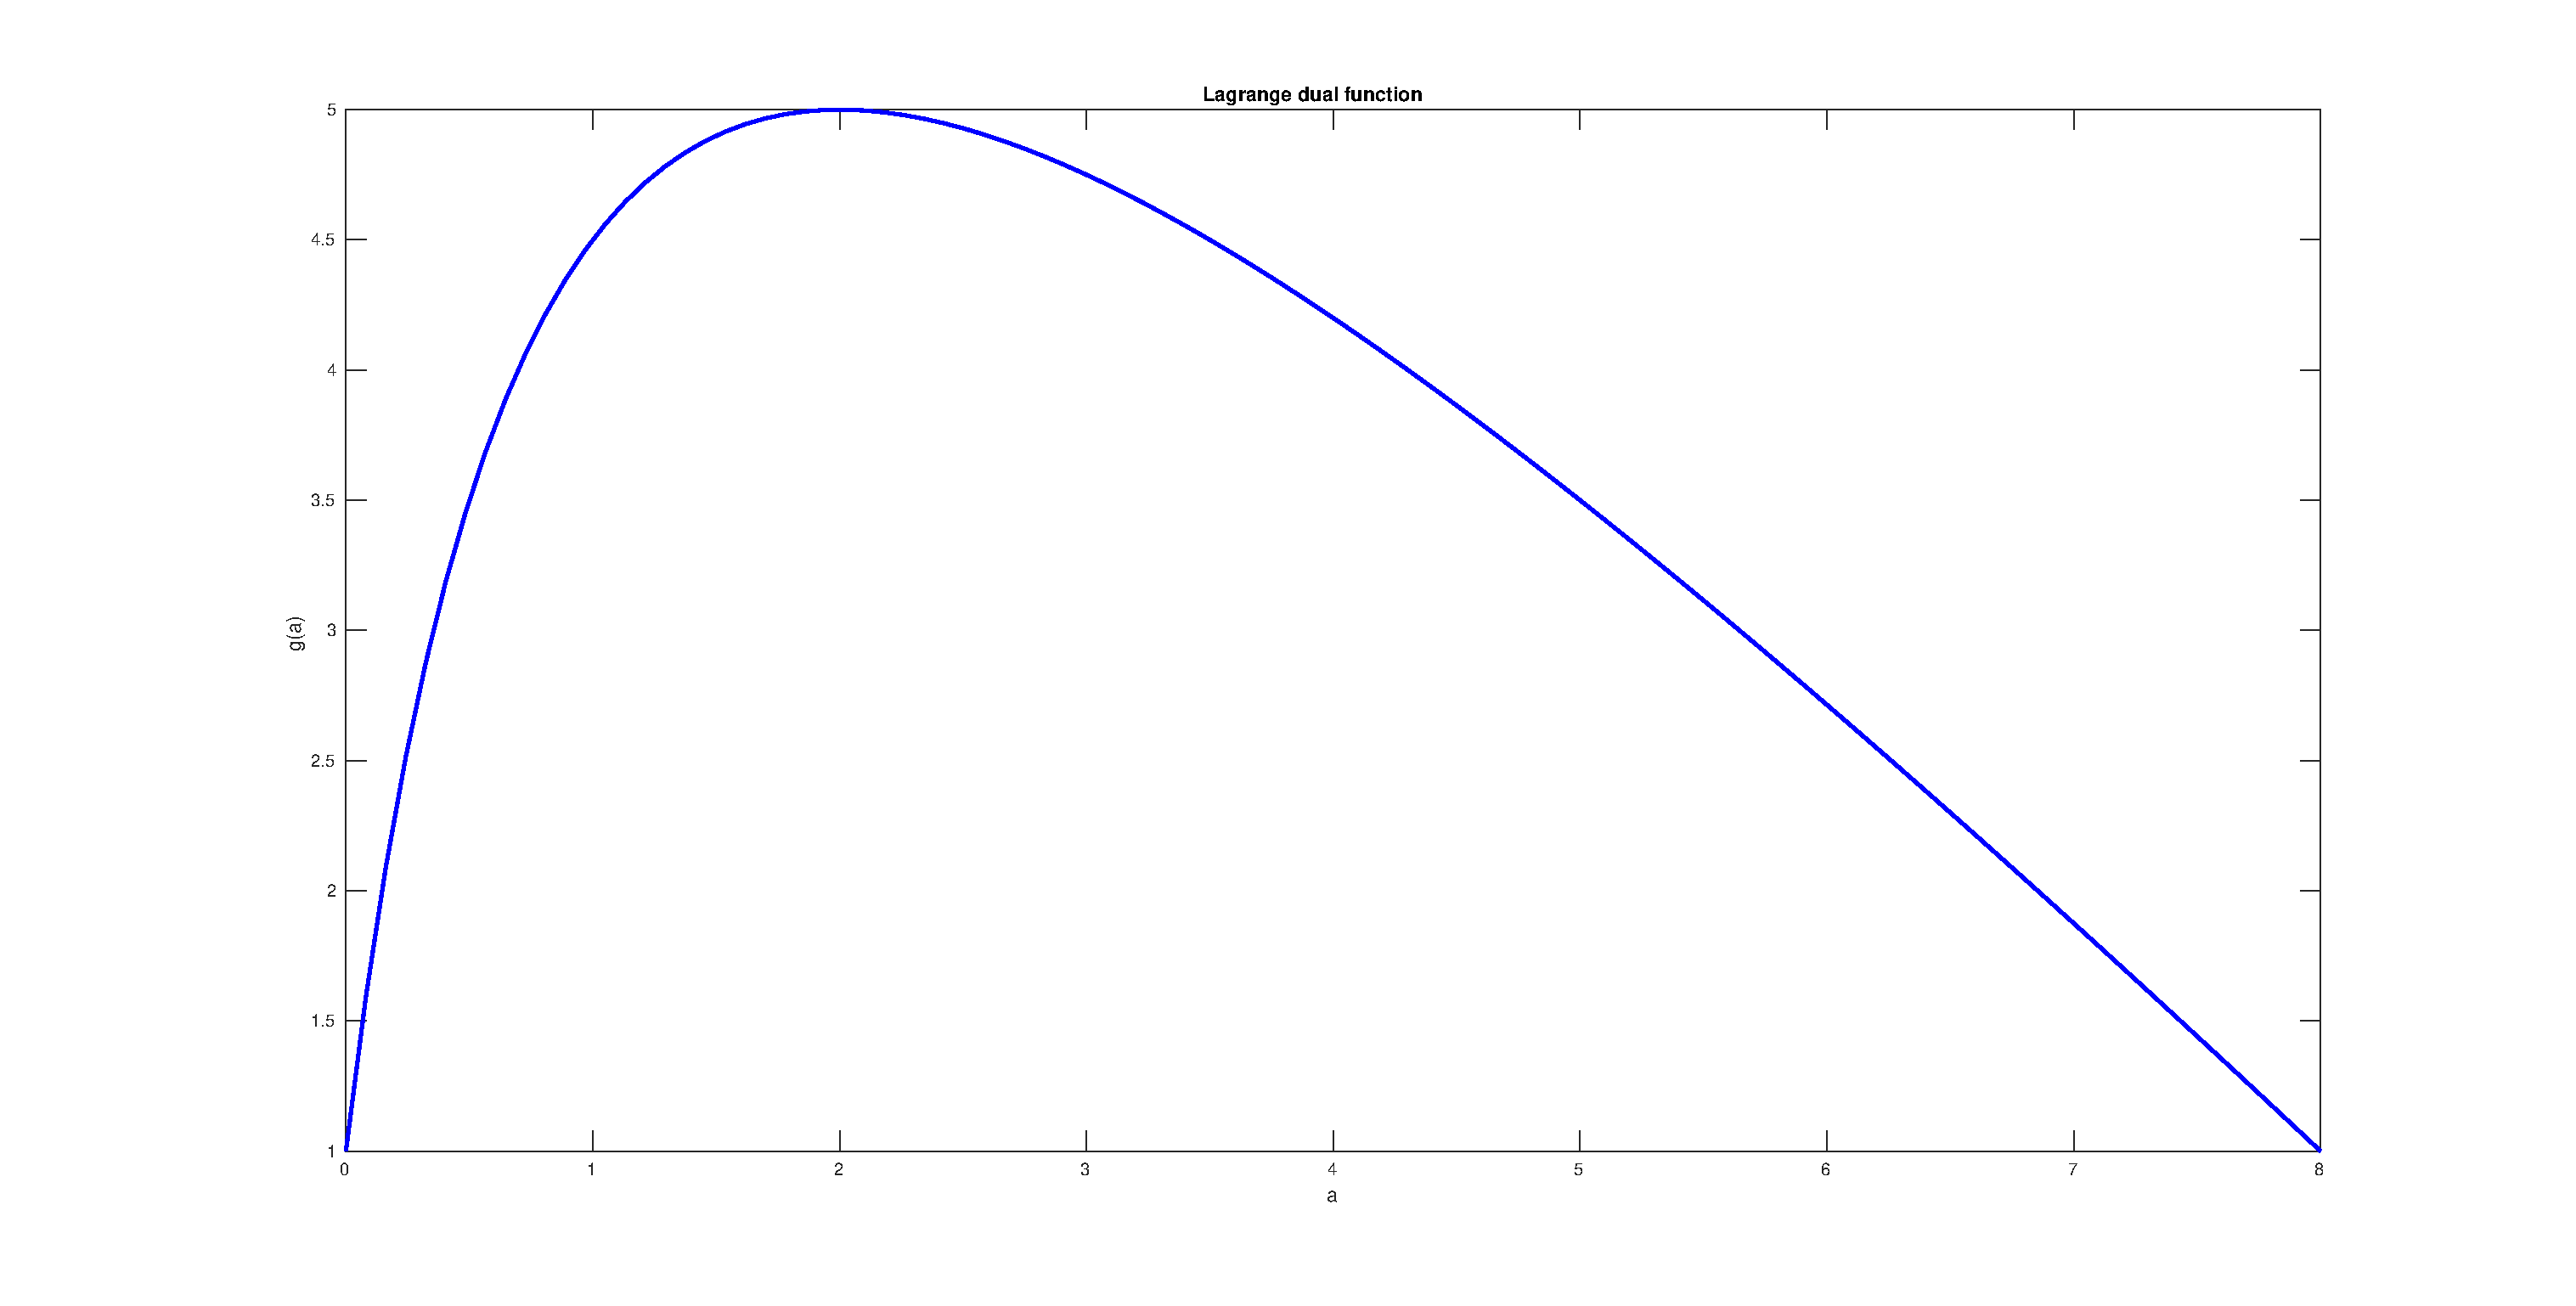
\includegraphics[width=\textwidth]{prob7}
 \caption{Lagrange dual function $g(\alpha)$.}
 \label{fig:dual}
\end{figure}

\section*{Problem 8}

\begin{equation}
 \alpha^\star = \arg \max_\alpha g(\alpha) 
\end{equation}
\begin{equation}
 0 = \frac{\partial}{\partial \alpha} g(\alpha) = \frac{- \alpha^2 - 2 \alpha +8}{(1 + \alpha)^2} \text{ and } \alpha \geq 0
\end{equation}

The dual optimal solution $\alpha^\star = 2$ and $g(\alpha^\star) = 5$.

\section*{Problem 9}

\begin{equation}
 x^\star = \frac{3 \alpha^\star}{1 + \alpha^\star} = \frac{6}{1 + 2} = 2
\end{equation}

The optimal solution is given by $f_0(x^\star) = 5$, which is equal to the dual optimal value.

\section*{Problem 10}

The constraint $f_1$ is active. We can see it also on the plot of the primal problem in Fig. \ref{optimizationprob}, since the feasible region is bounded by the zero-crossings of this constraint and the objective function attains its minimum at one of them.

  
\end{document}
